\documentclass[11pt,a4paper]{article}
\usepackage[utf8]{inputenc}
\usepackage{geometry}
\usepackage{graphicx}
\usepackage{booktabs}
\usepackage{hyperref}
\usepackage{float}
\geometry{margin=1in}

\title{Assignment 3 \\ Experimentation and Analysis of Chain Reaction AI Agents}
\author{Gourove Roy}
\date{\today}

\begin{document}

\maketitle

\section{Introduction}
Chain Reaction is a turn-based strategy game played on a $9\times6$ grid (default), where players take turns placing orbs in cells. When a cell exceeds its critical mass, it explodes, sending orbs to neighboring cells and potentially triggering chain reactions. The objective is to eliminate all of the opponent's orbs. This report analyzes the performance of different AI agents (Random, Minimax with various depths and heuristics) and compares them with human play.

\section{Experimental Setup}
\begin{itemize}
  \item \textbf{Board size:} $9\times6$ (default).
  \item \textbf{Agents:}
    \begin{itemize}
      \item \textbf{Random:} Selects moves randomly.
      \item \textbf{Minimax:} Uses minimax with alpha-beta pruning and custom heuristics.
    \end{itemize}
  \item \textbf{Depths tested:} 1, 2, 3, 4.
  \item \textbf{Heuristics:}
    \begin{itemize}
      \item \textbf{Heuristic 0:} Simple Orb-Count Difference.
      \item \textbf{Heuristic 1:} Weighted by Critical Mass Proximity.
      \item \textbf{Heuristic 2:} Chain-Reaction Potential.
      \item \textbf{Heuristic 3:} Board Control (Corners and Edges).
      \item \textbf{Heuristic 4:} Mobility / Legal Move Count.
      \item \textbf{Heuristic 5:} Linear Combination (Mixture) of All Heuristics.
      \item \textbf{Heuristic 6:} Adaptive Best Heuristic (Max Ensemble).
    \end{itemize}
  \item \textbf{Time measurement:} Average time per move (from AI logs), total game time.
  \item \textbf{Matches:}
    \begin{enumerate}
      \item Random vs. Minimax varying depths and heuristics.
      \item Minimax depth d1 vs Minimax depth d2 (same heuristic)
      \item Minimax heuristic h1 vs Minimax heuristic h2 (fixed depth)
      \item Human vs. AI (minimax)
    \end{enumerate}
\end{itemize}

\section{Results}
\subsection{Detailed Comparison Tables}
\begin{figure}[H]
  \centering
  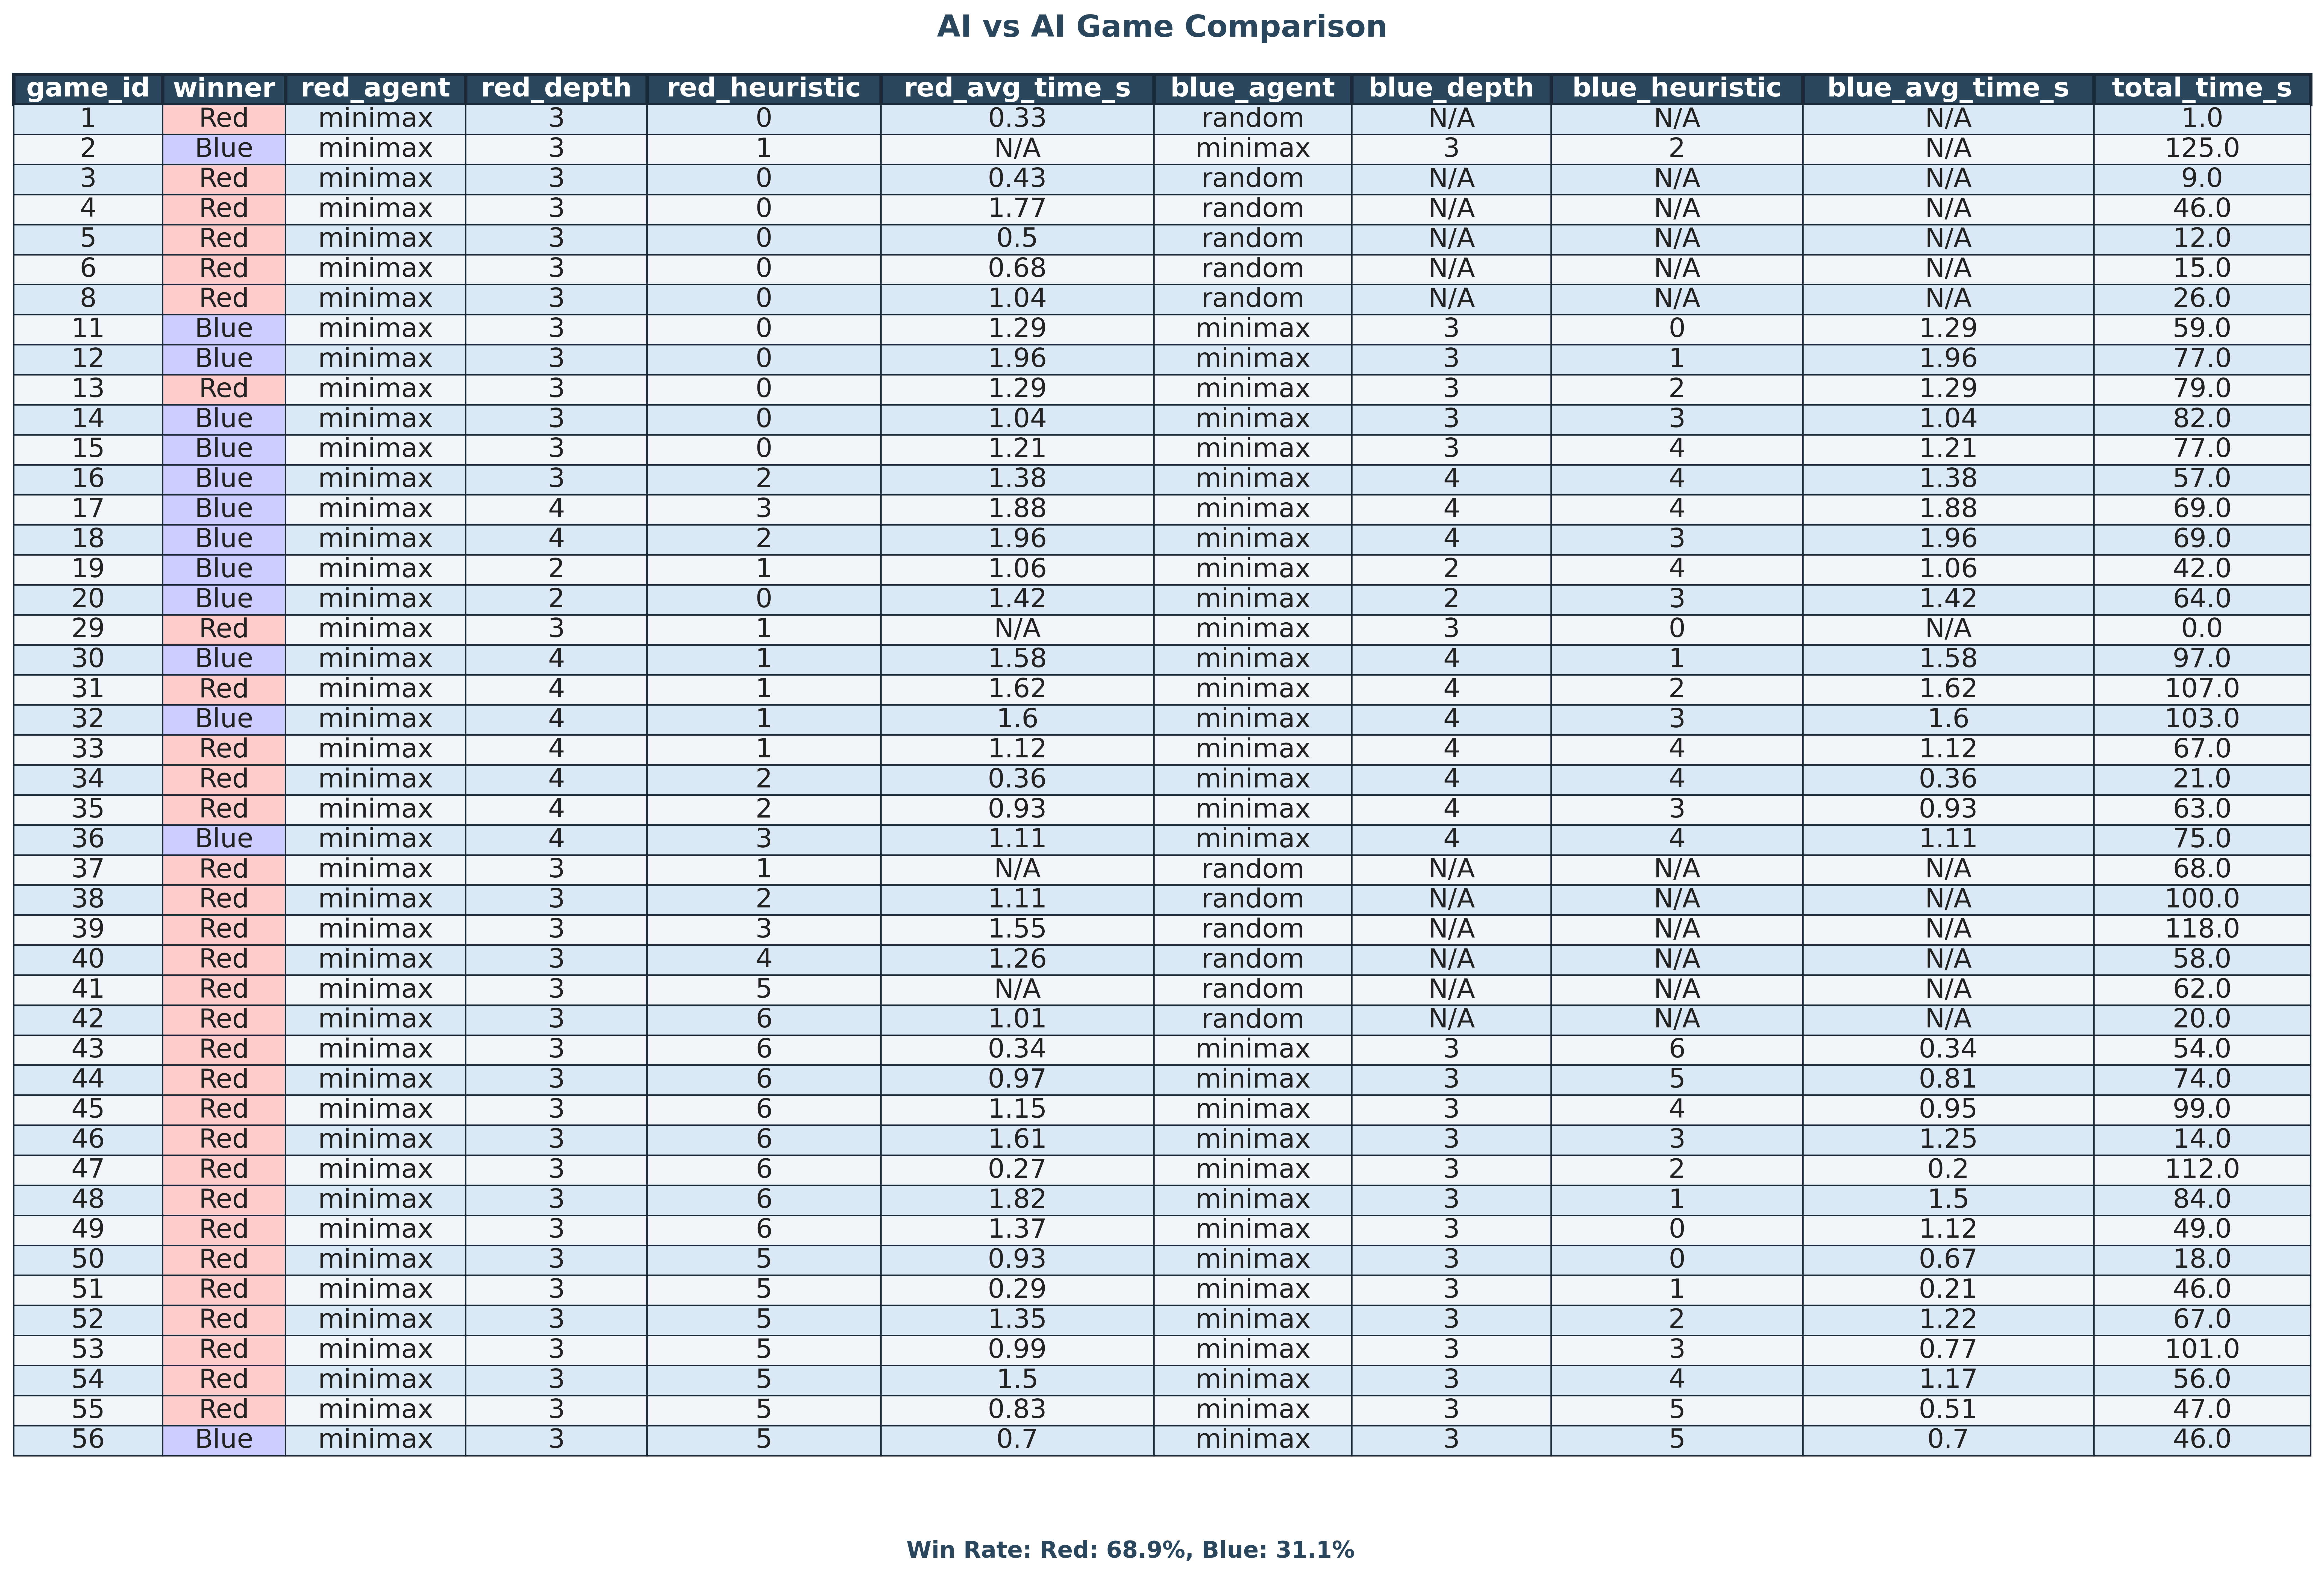
\includegraphics[width=\textwidth,height=0.55\textheight]{analysis/ai_vs_ai_table.png}
  \caption{AI vs AI Game Comparison Table with Win Rate}
\end{figure}

\begin{figure}[H]
  \centering
  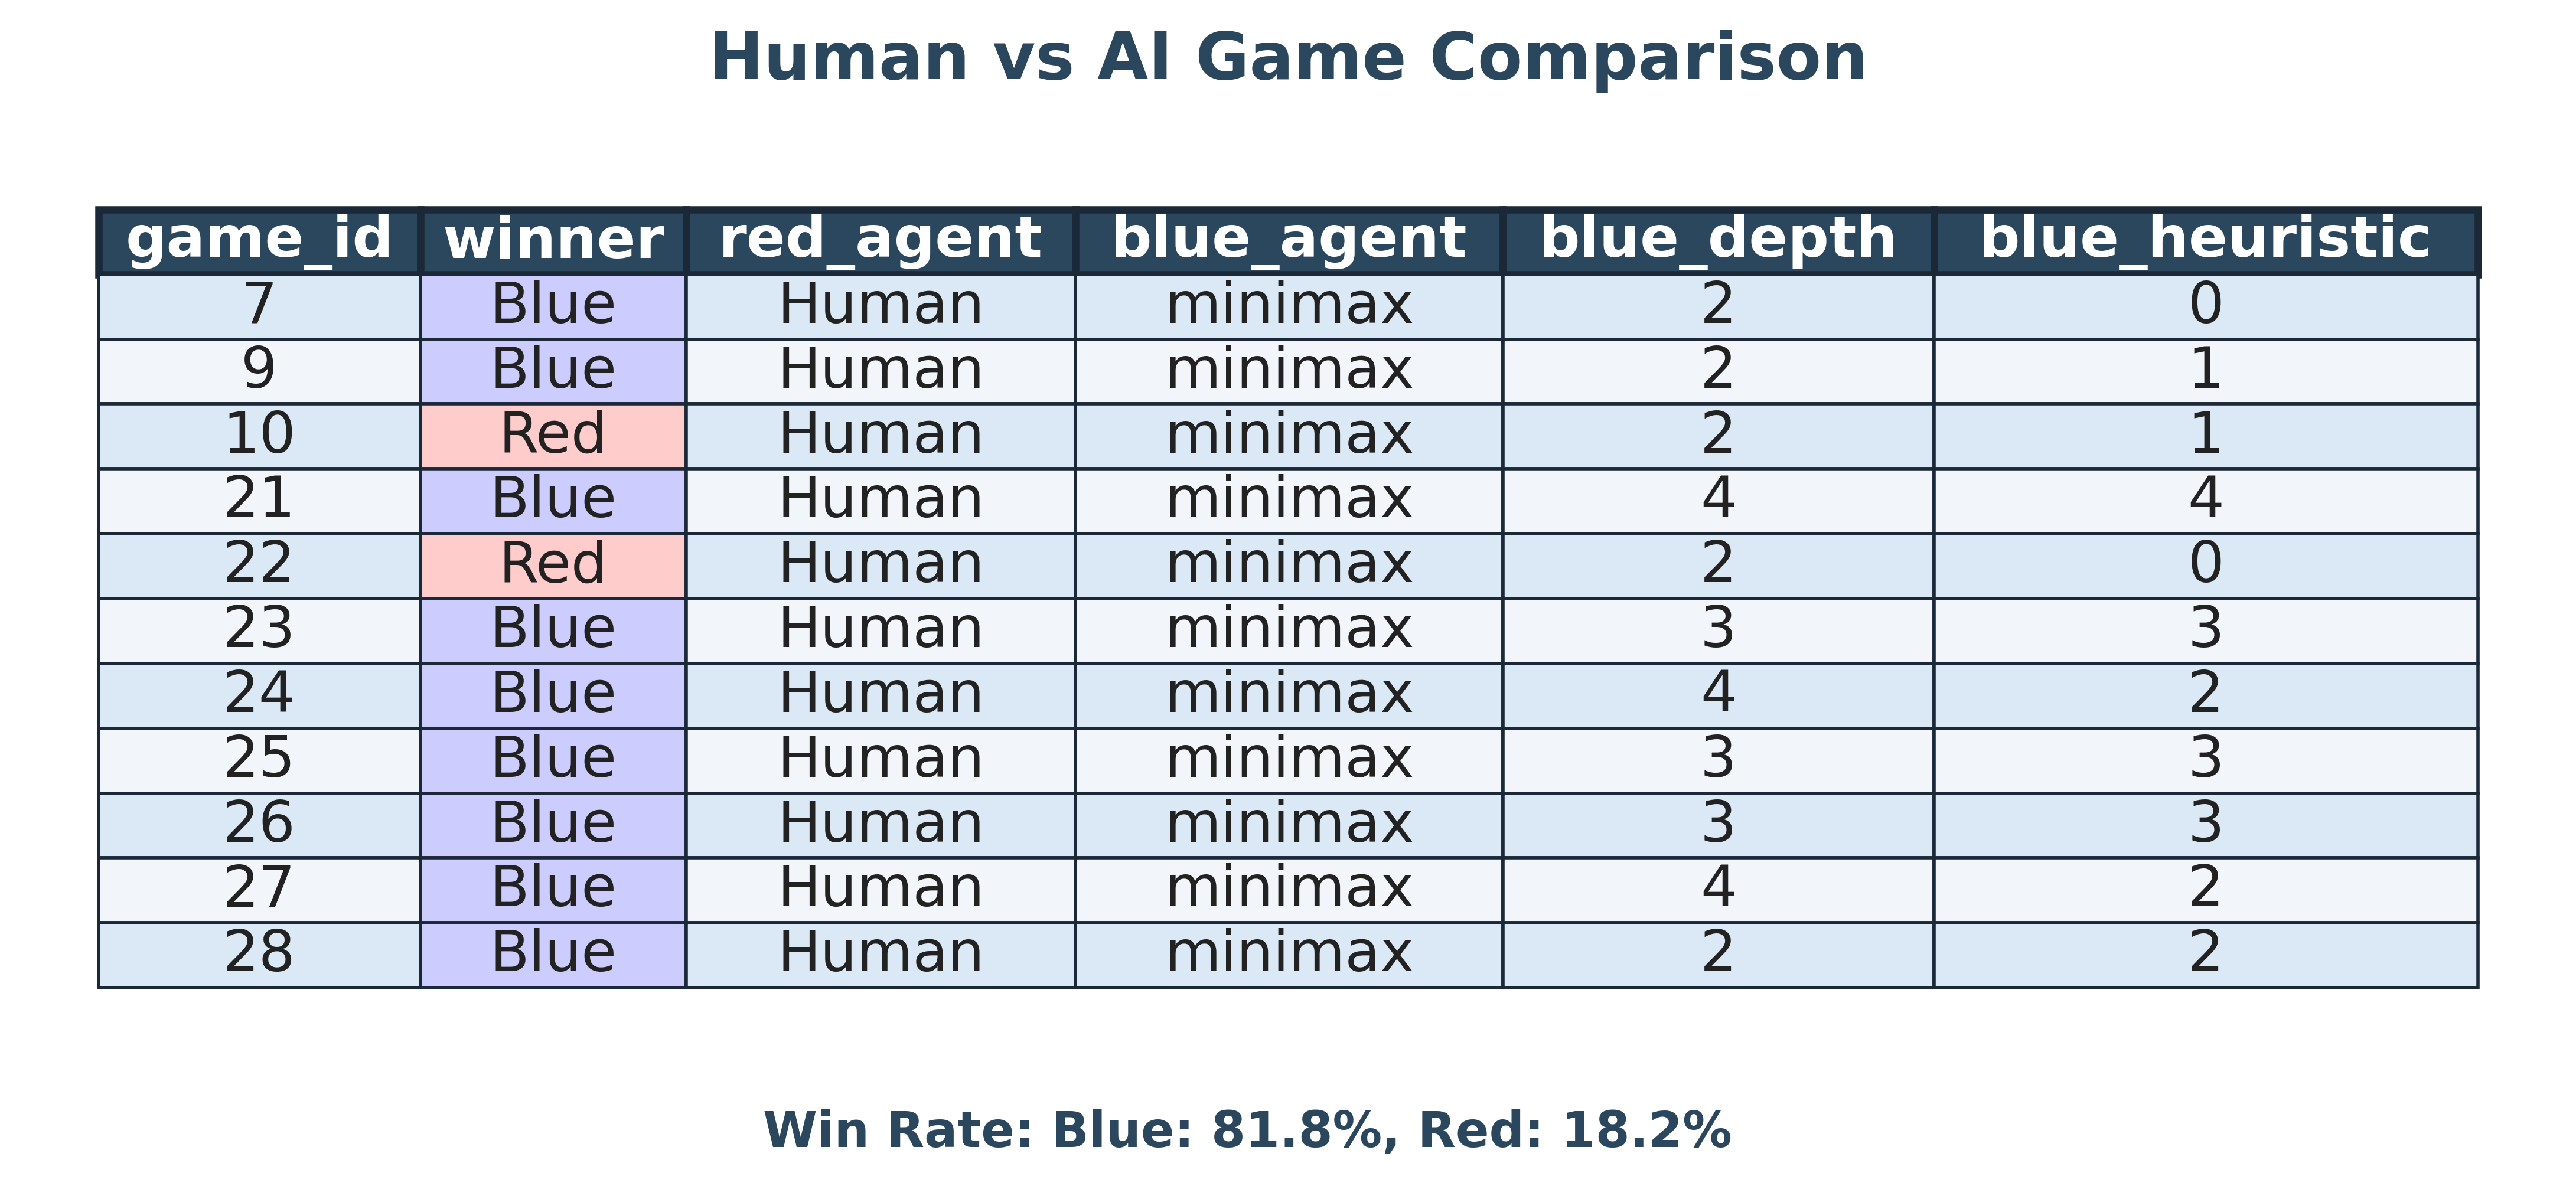
\includegraphics[width=0.8\textwidth]{analysis/human_vs_ai_table.png}
  \caption{Human vs AI Game Comparison Table with Win Rate}
\end{figure}

\subsection{Heuristic Performance Statistics}

To evaluate which heuristic performed best, we analyzed all AI vs AI matches (excluding Human vs AI). For each heuristic (0--6), we counted the number of games played, number of wins, and calculated the win rate. If any agent was random, we compared heuristics based on average total game time.

\begin{table}[H]
\centering
\begin{tabular}{cccc}
\toprule
\textbf{Heuristic} & \textbf{Games Played} & \textbf{Wins} & \textbf{Win Rate (\%)} \\
\midrule
0 & 32 & 11 & 34.4 \\
1 & 17 & 6 & 35.3 \\
2 & 18 & 5 & 27.8 \\
3 & 18 & 3 & 16.7 \\
4 & 18 & 7 & 38.9 \\
5 & 13 & 6 & 46.2 \\
6 & 10 & 8 & 80.0 \\
\bottomrule
\end{tabular}
\caption{Heuristic-wise performance in AI vs AI matches (win rate = wins/games played).}
\end{table}

\begin{table}[H]
\centering
\begin{tabular}{ccc}
\toprule
\textbf{Heuristic} & \textbf{Description} & \textbf{Avg Time vs Random (s)} \\
\midrule
0 & Orb-Count Difference & 18.2 \\
1 & Critical Mass Proximity & 68.0 \\
2 & Chain-Reaction Potential & 100.0 \\
3 & Board Control (Corners/Edges) & 118.0 \\
4 & Mobility / Legal Move Count & 58.0 \\
5 & Mixture of All Heuristics & 62.0 \\
6 & Adaptive Best (Max Ensemble) & 41.0 \\
\bottomrule
\end{tabular}
\caption{Average total game time for minimax vs random agent by heuristic.}
\end{table}

\textbf{Summary:}
\begin{itemize}
    \item \textbf{Heuristic 6} (Adaptive Best/Max Ensemble) achieved the highest win rate (80\%) among all AI vs AI matches.
    \item \textbf{Heuristic 5} (Mixture) also performed strongly (46.2\% win rate).
    \item \textbf{Heuristic 4} (Mobility) and \textbf{Heuristic 1} (Critical Mass Proximity) had solid win rates (38.9\% and 35.3\%).
    \item \textbf{Heuristic 0} (Orb-Count Difference) was the most used, with a win rate of 34.4\%, and was the fastest against random (18.2s).
    \item Heuristics 2 and 3 had lower win rates in these experiments.
\end{itemize}

\textbf{Conclusion:} Heuristic 6 (Adaptive Best) performed best by win rate in AI vs AI matches. Heuristic 0 is fastest and most effective against random. Mixture (Heuristic 5) is also a strong choice.
\pagebreak
\section{Discussion}
The experiments show that:
\begin{itemize}
  \item \textbf{Minimax} (even at depth 2) is significantly stronger than the random agent.
  \item Increasing \textbf{depth} improves win rate but also increases computation time per move.
  \item \textbf{Heuristic 1} (Weighted by Critical Mass Proximity) can outperform the basic heuristic in some matchups, especially in controlling corners and edges.
  \item The AI (minimax) consistently outperforms human players at default settings.
\end{itemize}

\subsection*{Trade-offs Observed:}
\begin{itemize}
  \item \textbf{Computational Complexity:}
    \begin{itemize}
      \item Simpler heuristics such as \textbf{Heuristic 0} (Orb-Count Difference) and \textbf{Heuristic 1} (Critical Mass Proximity) are computationally efficient, as they only require a single pass over the board.
      \item More advanced heuristics like \textbf{Heuristic 2} (Chain-Reaction Potential), \textbf{Heuristic 3} (Board Control), and \textbf{Heuristic 4} (Mobility) involve additional logic such as neighbor checks or legal move counting, increasing per-move computation time.
      \item Using deeper search (higher depth) with complex heuristics can significantly increase total computation time, making real-time play less practical.
    \end{itemize}
  \item \textbf{Strategic Depth:}
    \begin{itemize}
      \item Simple heuristics (e.g., Orb-Count) may miss tactical opportunities, such as setting up chain reactions or controlling key board positions.
      \item Heuristics that consider proximity to explosion (\textbf{Heuristic 1}) or chain-reaction potential (\textbf{Heuristic 2}) provide greater strategic awareness, allowing the AI to anticipate and exploit multi-step tactics.
      \item Board control (\textbf{Heuristic 3}) and mobility (\textbf{Heuristic 4}) encourage the AI to occupy stable positions and maximize available moves, which can be crucial in the late game.
      \item There is a trade-off: more sophisticated heuristics can improve decision quality but may not always translate to higher win rates if not paired with sufficient search depth.
    \end{itemize}
\end{itemize}

Trade-offs between depth and speed are evident: depth 4 offers higher win rates but may not be practical for real-time play due to longer move times.

\section{Conclusion}
Minimax with alpha-beta pruning and well-designed heuristics provides a strong AI for Chain Reaction. Depth and heuristic choice both impact performance and speed. Future improvements could include iterative deepening, transposition tables, or adaptive heuristics for even stronger and faster AI.

\end{document}
